\clearpage
\subsection{Pass by Reference} % (fold)
\label{sub:pass_by_reference}

As with other Variables, you can pass an array to Functions and Procedures. The only real difference is that the array can potentially store significantly more data than other variables. When the array is passed by value each of its elements must be passed to the Parameter. Passing the parameter in this way means that there will be two copies of the data in memory, which takes more time and more memory.

You should avoid passing arrays by value, and instead pass them by reference. When passed by reference the array itself is passed across. This gives the called Function or Procedure access to the data, but does not require that the values be copied across.

One issue with always using pass by reference is that it allows the called code to change the data in array you are passing across. This can be useful, but at other times you want to pass the data across without allowing it to be changed by the called code. Both C and Pascal allow you to indicate that the data you are passing should be passed by reference, but that it cannot be changed in the called code.

\begin{figure}[h]
   \centering
   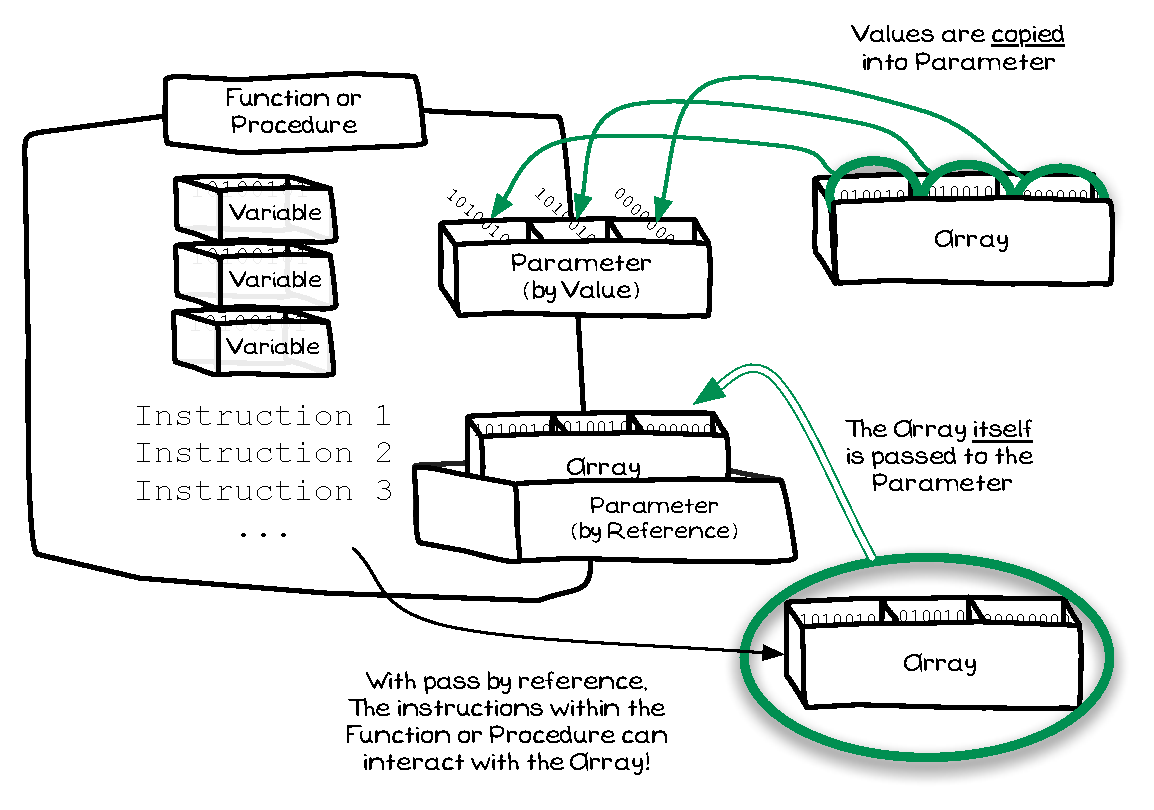
\includegraphics[width=0.9\textwidth]{./topics/arrays/diagrams/ByRefByVal} 
   \caption{Arrays should always be passed by Reference}
   \label{fig:array-by-ref-by-val}
\end{figure}

\mynote{
\begin{itemize}
  \item Pass by Reference and Pass by Value are \textbf{terms} that explain how data is passed to a Parameter.
  \item With arrays you should always use \emph{Pass by Reference}. This will be faster and take less memory.
  \item The \textbf{const} keyword can be used to indicate that the parameter should not be able to be changed by the called code.
\end{itemize}
}

\csection{In C you cannot pass an array by value, instead all arrays are passed by reference automatically by the language.}

% subsection passing_by_reference (end)